\section{Systeme und Methoden}

\subsection{Biometrische Systeme}

\frame{\frametitle{Biometrische Systeme}
Biometrische Systeme nutzen zur Identifizierung biometrische Daten, welche folgenden Ansprüchen genügen müssen.

\begin{itemize}
\item Körperliche Charakteristika sollte sich zu Lebenszeiten nicht ändern.
\item Körperliche Charakteristika muss eindeutig einer Person zugeordnet werden können.
\item Körperliche Charakteristika sollte einfach, schnell und mit möglichst günstigen Geräten ermittelt werden können.
\item Die Daten müssen einfach, automatisch und schnell überprüft werden können.
\end{itemize}
}

\frame{\frametitle{Biometrische Systeme}
Des weiteren können folgende Punkte hilfreich sein um eine erfolgreiche biometrische Erkennung durchzuführen.

\begin{itemize}
\item Sie sollte so simpel sein, das auch angelernte Personen schnell eine fehlerfreie Identifizierung durchführen können.
\item Die Mithilfe der zu identifizierenden Person sollte nicht nötig sein.
\item Nutzung von gespeicherten Daten, wie zum Beispiel Sprachsample.
\end{itemize}
}


\frame{\frametitle{Biometrische Systeme}

\begin{center}
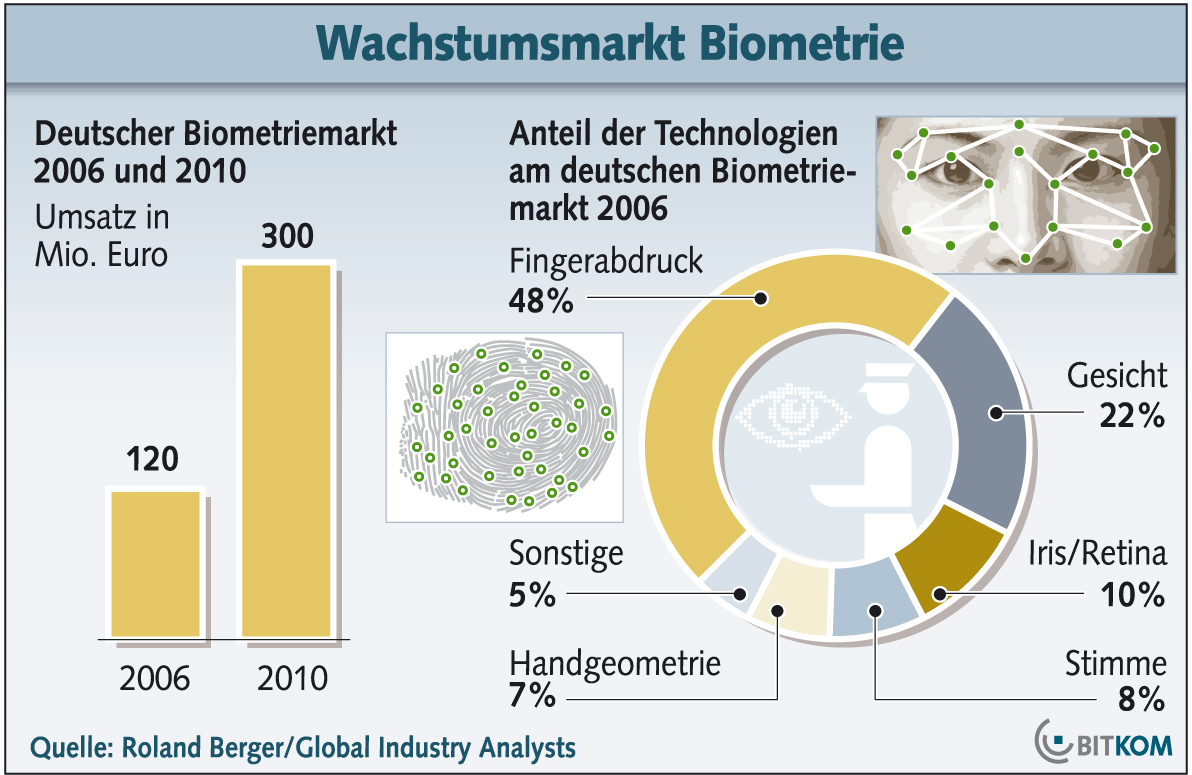
\includegraphics[scale=0.75]{pic/Biometrie}
\end{center}

}

\subsection{Technische Systeme}

\subsubsection{Aktive Medien}
\frame{\frametitle{Aktive Medien}
Bei aktiven Medien findet eine Bidirektionale Kommunikation statt. Dazu kann ein spezielles Prüfgerät eingesetzt werden oder die Kommunikation läuft wie bei dem bekanntesten aktiven \emph{\textbf{Token}} dem Smartphone oder Mobiltelefon über Bluetooth.\\[2ex]

Weitere aktive Tokens sind aktive RFID Transponder oder Chip-Karten.
}

\subsubsection{Passive Medien}
\frame{\frametitle{Passive Medien}
\begin{itemize}
\item USB-Token
\item Smartcard
\item Trusted Platform Modules (TPM)
\item RFID
\end{itemize}
}

\subsection{Software Lösungen}
\frame{\frametitle{Software Lösungen}
\begin{itemize}
\item Benutzerkonten
\begin{itemize}
\item Betriebssysteme
\item Datenbanksysteme
\item Online Dienste
\end{itemize}
\item Directories
\item Cookies
\end{itemize}
}